\documentclass[11pt]{article}

\usepackage[margin=1in]{geometry}
\usepackage[T1]{fontenc}
\usepackage{lmodern}
\usepackage{microtype}
\usepackage{amsmath, amssymb}
\usepackage{booktabs}
\usepackage{array}
\usepackage{tabularx}
\usepackage{tikz}
\usetikzlibrary{arrows.meta, positioning, shapes.geometric, calc, decorations.pathreplacing, backgrounds}
\usepackage{float}
\usepackage[hidelinks]{hyperref}
\usepackage{caption}
\usepackage{xcolor}
\usepackage{enumitem}
\usepackage[round]{natbib}

\setlength{\parskip}{0.5em}
\setlength{\parindent}{0pt}

\newcommand{\ticustart}{t^{\text{ICU}_1,\text{start}}}
\newcommand{\ticuend}{t^{\text{ICU}_1,\text{end}}}

\title{\textbf{FLAIR Task Schematic} \\[0.3em]
       Unplanned ICU Readmission (Task T5)}
\author{FLAIR Benchmark}
\date{\today}

\begin{document}
\maketitle

\begin{abstract}
\noindent We specify the FLAIR unplanned ICU readmission task: at the end
of a patient's first ICU stay, predict whether the patient will return to
the ICU later in the \emph{same} hospitalization through an unplanned path.
The signal is derived entirely from the CLIF \texttt{ADT} location history.
A \emph{planned} return --- ICU $\to$ Procedural $\to$ ICU, e.g. a trip to
the OR or cath lab and back --- is not counted: the procedural segment is
removed and the two ICU stays merge into one. The task is one-per-stay
(exactly one prediction per surviving hospitalization), in contrast to the
continuous, one-per-window FLAIR tasks.
\end{abstract}

\section{FLAIR operational definition}
\label{sec:def}

\subsection{Anchors and windows}

Let $H_i$ denote a hospitalization. From the CLIF \texttt{ADT} table we
compute (see \verb|compute_readmission_timing|) a merged location sequence
and, from it, the first ICU stay window
$[\ticustart_i,\, \ticuend_i]$ and the start time of a second ICU stay
(if any).

\begin{description}[leftmargin=2em, style=nextline]

\item[Location standardization.]
Each \texttt{adt.location\_category} is lowercased and mapped to a coarse
bucket \texttt{std\_location} $\in \{$ICU, Ward, ER, Procedural, Other$\}$
via \texttt{LOCATION\_MAPPING}. Stepdown, L\&D, hospice, psych, rehab,
radiology, dialysis, and other all map to \texttt{Other}.

\item[Procedural-sandwich removal (planned readmission).]
A row with \texttt{std\_location} $=$ Procedural whose immediate
predecessor and successor (within $H_i$, ordered by \texttt{in\_dttm}) are
both ICU is deleted. This collapses ICU $\to$ Procedural $\to$ ICU into a
single ICU stay: a planned procedural excursion is \emph{not} a
readmission.

\item[Consecutive-location merge.]
After sandwich removal, consecutive rows with the same
\texttt{std\_location} are merged into one location group spanning
$[\min(\texttt{in\_dttm}),\, \max(\texttt{out\_dttm})]$. Back-to-back ICU
ADT rows therefore form a single ICU stay.

\item[First / second ICU stay.]
Rank the merged ICU groups of $H_i$ by \texttt{in\_dttm}. Group 1 yields
$\ticustart_i, \ticuend_i$. Group 2, if present, is the unplanned
readmission with start \texttt{second\_icu\_start\_time}.

\item[Prediction time.]
$\text{prediction\_dttm}_i = \ticuend_i$ (decision made at first-ICU
discharge).

\item[Input window.]
$[\,\text{window\_start}_i,\, \text{window\_end}_i\,] =
[\ticustart_i,\, \ticuend_i]$ --- the entire first ICU stay
(variable length; no fixed lookback).

\item[Label (\texttt{label\_icu\_readmission}).]
$y_i = \mathbb{1}\!\left[\texttt{second\_icu\_start\_time}_i \neq
\varnothing\right]$.

\end{description}

\subsection{Cohort}

\begin{itemize}[leftmargin=2em]
  \item Age at admission $\ge 18$ with valid \texttt{admission\_dttm} and
        \texttt{discharge\_dttm}.
  \item $\geq 1$ ICU ADT record (first ICU stay defined).
  \item \textbf{Exclude} hospitalizations with no ICU data (no first ICU
        stay) --- realized as an inner join with the timing table.
  \item \textbf{Exclude} death during the first ICU stay
        (\texttt{death\_dttm} $\in [\ticustart_i, \ticuend_i]$): the
        readmission outcome is undefined.
  \item \textbf{Exclude} direct ICU discharge (the last merged location is
        ICU): there is no opportunity to readmit.
  \item \textbf{Exclude} a first ICU stay shorter than
        \texttt{MIN\_ICU\_STAY\_HOURS} $= 1$ hour.
  \item \textbf{Exclude} an intermediate ER visit (an ER location after the
        first location), which confounds the planned/unplanned distinction.
\end{itemize}

\subsection{CLIF tables and categories used}
\label{sec:t5-clif}

Task~T5 reads three CLIF v2.1 tables. The entire readmission signal is the
\texttt{adt.location\_category} sequence; \texttt{hospitalization} and
\texttt{patient} provide cohort filters, the death timestamp, and
demographics.

\begin{table}[H]
\centering
\small
\begin{tabular}{@{}llp{6.6cm}@{}}
\toprule
\textbf{CLIF table} & \textbf{Category column} & \textbf{Use} \\
\midrule
\texttt{hospitalization} & ---                       & cohort/demographics join; \texttt{age\_at\_admission}, valid dates \\
\texttt{patient}         & ---                       & demographics join; \texttt{death\_dttm} for the death exclusion \\
\texttt{adt}             & \texttt{location\_category} & merged into ICU / Ward / ER / Procedural / Other; sole readmission signal \\
\bottomrule
\end{tabular}
\caption{CLIF surface for Task~T5. No \texttt{labs}, \texttt{vitals}, or
medication tables are read --- the task is ADT-only.}
\end{table}

Columns selected from each table:
\begin{itemize}[leftmargin=2em, itemsep=0pt]
  \item \texttt{hospitalization}: \texttt{hospitalization\_id},
        \texttt{patient\_id}, \texttt{admission\_dttm},
        \texttt{discharge\_dttm}, \texttt{age\_at\_admission},
        \texttt{discharge\_category}.
  \item \texttt{patient}: \texttt{patient\_id}, \texttt{sex\_category},
        \texttt{race\_category}, \texttt{ethnicity\_category},
        \texttt{death\_dttm}.
  \item \texttt{adt}: \texttt{hospitalization\_id},
        \texttt{location\_category}, \texttt{in\_dttm}, \texttt{out\_dttm}.
\end{itemize}

\section{Algorithmic flow}
\label{sec:flow}

\begin{figure}[H]
\centering
\resizebox{\textwidth}{!}{% Algorithmic flowchart for the FLAIR unplanned ICU readmission build pipeline.

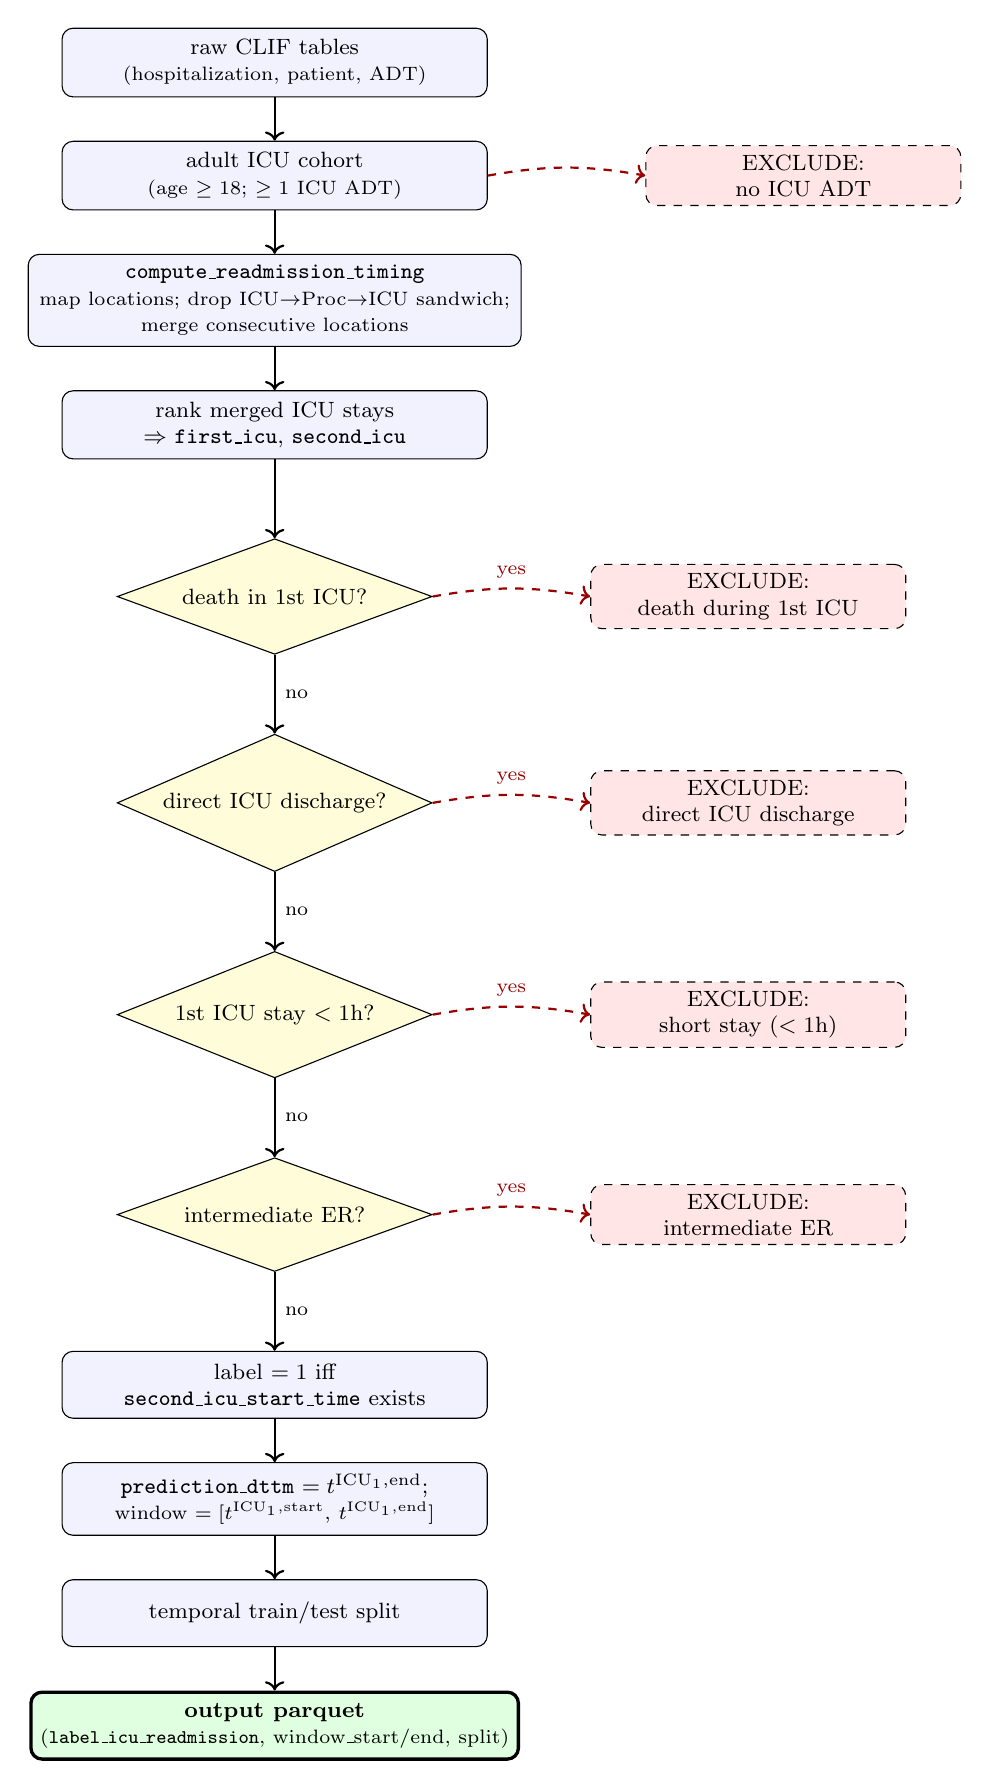
\begin{tikzpicture}[
    node distance=0.55cm and 0.7cm,
    every node/.style={font=\footnotesize, align=center},
    box/.style={draw, rounded corners, fill=blue!5,
                minimum width=5.4cm, minimum height=0.85cm, inner sep=4pt},
    dbox/.style={draw, diamond, aspect=2.2, fill=yellow!15,
                 minimum width=4.0cm, inner sep=2pt},
    excl/.style={draw, rounded corners, fill=red!10, dashed,
                 minimum width=4.0cm, minimum height=0.7cm},
    outbox/.style={draw, rounded corners, fill=green!12, very thick,
                minimum width=5.4cm, minimum height=0.85cm},
    arrow/.style={->, thick},
    sidearrow/.style={->, thick, red!60!black, dashed},
]
    % main pipeline
    \node[box] (raw) {raw CLIF tables\\\scriptsize(hospitalization, patient, ADT)};
    \node[box, below=of raw] (cohort)
        {adult ICU cohort\\\scriptsize(age $\geq 18$; $\geq 1$ ICU ADT)};
    \node[box, below=of cohort] (timing)
        {\texttt{compute\_readmission\_timing}\\\scriptsize map locations; drop ICU$\to$Proc$\to$ICU
         sandwich;\\\scriptsize merge consecutive locations};
    \node[box, below=of timing] (rank)
        {rank merged ICU stays\\$\Rightarrow$ \texttt{first\_icu}, \texttt{second\_icu}};

    \node[dbox, below=1.0cm of rank] (death)
        {death in 1st ICU?};
    \node[dbox, below=1.0cm of death] (direct)
        {direct ICU discharge?};
    \node[dbox, below=1.0cm of direct] (short)
        {1st ICU stay $< 1$h?};
    \node[dbox, below=1.0cm of short] (er)
        {intermediate ER?};

    \node[box, below=1.0cm of er] (label)
        {label $= 1$ iff\\\texttt{second\_icu\_start\_time} exists};
    \node[box, below=of label] (window)
        {\texttt{prediction\_dttm} $= t^{\text{ICU}_1,\text{end}}$;\\\scriptsize window $= [t^{\text{ICU}_1,\text{start}},\, t^{\text{ICU}_1,\text{end}}]$};
    \node[box, below=of window] (split) {temporal train/test split};
    \node[outbox, below=of split] (parquet)
        {\textbf{output parquet}\\\scriptsize{(\texttt{label\_icu\_readmission}, window\_start/end, split)}};

    % exclusions on the right
    \node[excl, right=2.0cm of cohort] (exclNoIcu)
        {EXCLUDE:\\no ICU ADT};
    \node[excl, right=2.0cm of death] (exclDeath)
        {EXCLUDE:\\death during 1st ICU};
    \node[excl, right=2.0cm of direct] (exclDirect)
        {EXCLUDE:\\direct ICU discharge};
    \node[excl, right=2.0cm of short] (exclShort)
        {EXCLUDE:\\short stay ($<1$h)};
    \node[excl, right=2.0cm of er] (exclEr)
        {EXCLUDE:\\intermediate ER};

    % main arrows
    \draw[arrow] (raw) -- (cohort);
    \draw[arrow] (cohort) -- (timing);
    \draw[arrow] (timing) -- (rank);
    \draw[arrow] (rank) -- (death);
    \draw[arrow] (death) -- node[right, font=\scriptsize]{no} (direct);
    \draw[arrow] (direct) -- node[right, font=\scriptsize]{no} (short);
    \draw[arrow] (short) -- node[right, font=\scriptsize]{no} (er);
    \draw[arrow] (er) -- node[right, font=\scriptsize]{no} (label);
    \draw[arrow] (label) -- (window);
    \draw[arrow] (window) -- (split);
    \draw[arrow] (split) -- (parquet);

    % exclusion arrows
    \draw[sidearrow] (cohort.east) to[bend left=10] (exclNoIcu.west);
    \draw[sidearrow] (death.east) to[bend left=10]
        node[above, font=\scriptsize]{yes} (exclDeath.west);
    \draw[sidearrow] (direct.east) to[bend left=10]
        node[above, font=\scriptsize]{yes} (exclDirect.west);
    \draw[sidearrow] (short.east) to[bend left=10]
        node[above, font=\scriptsize]{yes} (exclShort.west);
    \draw[sidearrow] (er.east) to[bend left=10]
        node[above, font=\scriptsize]{yes} (exclEr.west);

\end{tikzpicture}
}
\caption{Build pipeline for Task~T5. Solid arrows: main flow. Dashed red
arrows: exclusions. The diamonds gate hospitalizations on death-in-ICU,
direct ICU discharge, short stay, and intermediate ER. The label is set by
the existence of a second merged ICU stay after procedural-sandwich removal
and consecutive-location merging.}
\label{fig:readmit-flow}
\end{figure}

Step-by-step prose:

\begin{enumerate}[leftmargin=2em]
  \item Load CLIF tables: \texttt{hospitalization}, \texttt{patient},
        \texttt{adt} via \texttt{base\_icu\_cohort}.
  \item Apply adult-ICU cohort filters (age, valid admission/discharge,
        $\geq 1$ ICU ADT).
  \item \texttt{compute\_readmission\_timing(adt)}: map locations; drop
        ICU $\to$ Procedural $\to$ ICU procedural rows; merge consecutive
        same-location rows; rank ICU groups to extract first/second ICU
        times; flag \texttt{is\_direct\_icu\_discharge} and
        \texttt{has\_intermediate\_er}.
  \item Inner-join timing into the cohort (drops no-ICU hospitalizations).
  \item Apply the four remaining exclusions: death during first ICU stay;
        direct ICU discharge; first ICU stay $<$ 1h; intermediate ER.
  \item Label $y_i = \mathbb{1}[\texttt{second\_icu\_start\_time} \neq
        \varnothing]$.
  \item Set \texttt{prediction\_dttm} $= \ticuend_i$ and the input window
        $[\ticustart_i, \ticuend_i]$.
  \item Assign temporal train/test split via
        \texttt{flair\_benchmark.\_split.assign\_split}, keyed on
        \texttt{prediction\_dttm}.
  \item Select \texttt{OUTPUT\_COLS} (the standard 10-column schema) and
        persist as parquet.
\end{enumerate}

\section{Design choices and rationale}
\label{sec:rationale}

\paragraph{Why ADT-only.}
ICU readmission is a movement event, fully observable from the CLIF
\texttt{ADT} location stream without labs, vitals, or notes. Restricting
the label to ADT keeps it portable across every CLIF site and avoids the
cadence/vocabulary assumptions that complicate the lab- and
medication-anchored tasks. The federated ML literature treats unplanned
ICU readmission as a structured-EHR target in exactly this spirit
\citep{rojas2018readmission}.

\paragraph{Why remove the procedural sandwich.}
A patient who leaves the ICU for a scheduled procedure (OR, cath lab,
interventional radiology) and returns has not been \emph{readmitted} in any
clinically meaningful sense --- the return was planned at the time of
transfer. Counting it would inflate the positive rate with non-events and
penalize a model for ``missing'' an outcome that carries no deterioration
signal. Collapsing ICU $\to$ Procedural $\to$ ICU to a single stay encodes
the planned/unplanned distinction at the cohort level. Procedural rows that
are \emph{not} bracketed by ICU on both sides are left in place.

\paragraph{Why one-per-stay (not continuous).}
Unlike the deterioration tasks, readmission has a single natural decision
point --- the moment of ICU discharge, when a clinician decides the patient
is stable enough to leave. A one-per-stay framing matches that decision and
keeps the label balanced (each hospitalization contributes one row rather
than many trivially-negative hourly rows).

\paragraph{Why the four post-cohort exclusions.}
Death in the first ICU stay makes the outcome undefined; a direct ICU
discharge removes any opportunity to readmit (a structurally guaranteed
negative); a sub-hour first ICU stay is typically an administrative
artifact rather than a true ICU course; an intermediate ER visit muddies
the planned/unplanned reading of a subsequent ICU entry. Each is a
deterministic ADT/timestamp predicate, applied in a fixed order.

\section{Out of scope}

\begin{itemize}[leftmargin=2em]
  \item Cross-hospitalization (30-day) ICU or hospital readmission.
  \item Third and later ICU readmissions within a stay.
  \item Time-to-readmission (survival) labels.
  \item ICD- or problem-list--based planned/unplanned adjudication
        (we use ADT location categories only).
  \item Input feature design.
\end{itemize}

\bibliographystyle{plainnat}
\bibliography{references}

\end{document}
